
  Map\footnote{
    W. Hirsch, S. Smale, Introduction to Chaos.
} $f$ is \textbf{chaotic}, if \\
\begin{itemize}
    \iitem{$f$ \textbf{sensitive} to the initial conditions.}
    \iitem{periodic orbits are dense everywhere;}
    \iitem{orbits are mixed;}
\end{itemize}

% \vspace{-5mm}

\begin{figure}[h]
    \begin{minipage}[h]{0.49\linewidth}
        \center{
        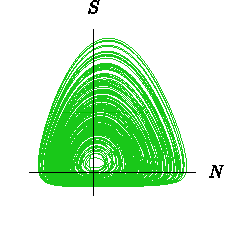
\includegraphics[width=0.7\linewidth]{figures/attractor.pdf}
        \\ 
        \vspace{-5mm} 
        Dense mixed orbits example}
    \end{minipage}
    \hfill
    \begin{minipage}[h]{0.49\linewidth}
        \center{
        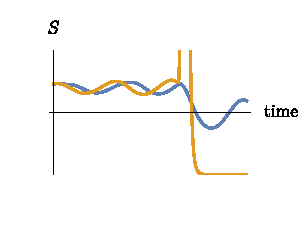
\includegraphics[width=0.98\linewidth]{figures/ics.pdf}
        \\ 
        \vspace{-5mm} 
        Sensitivity example}
    \end{minipage}
\end{figure}

% \begin{figure}[h]
%     \centering
%     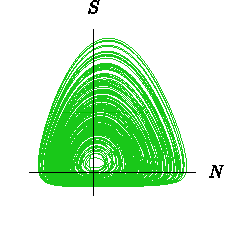
\includegraphics[width=0.35\textwidth]{figures/attractor.pdf}
%     \hspace{5 mm}
%     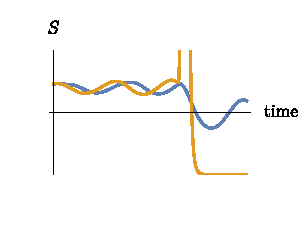
\includegraphics[width=0.49\textwidth]{figures/ics.pdf}
%     %\caption{}
%     %\label{fig:}
% \end{figure}


% подписать графики